% !TEX encoding = UTF-8
% !TEX TS-program = pdflatex
% !TEX root = ../tesi.tex

%**************************************************************
\chapter{Svolgimento}
\label{cap:svolgimento}
%**************************************************************

\intro{Il presente capitolo descrive le varie fasi dello sviluppo dell'applicazione}

\section{Pianificazione}
	Come modello per la gestione del progetto ho adottato la metodologia \gls{agileg}. Tale
	modello mi ha permesso di adottare una certa flessibilità e velocità nel rispondere alle
	esigenze e ai feedback del Dipartimento di Amministrazione.
	
	Il modello Agile prevede iterazioni continue, della durata massima di due settimane,
	entro le quali si susseguono attività di:
	\begin{enumerate}
		\item analisi dei requisiti che emergono dall’interazione con il cliente, in questo caso il tutor aziendale e il Dipartimento di Amministrazione;
		\item pianificazione delle funzionalità da includere nello sprint, suddivisione in task e loro assegnazione ai membri del team;
		\item progettazione delle funzionalità da implementare nell’iterazione corrente;
		\item codifica e sviluppo delle funzionalità previste;
		\item verifica;
		\item rilascio;
		\item monitoraggio continuo e verifica dello stato dell’applicazione.
	\end{enumerate}

		\begin{figure}
			\centering
			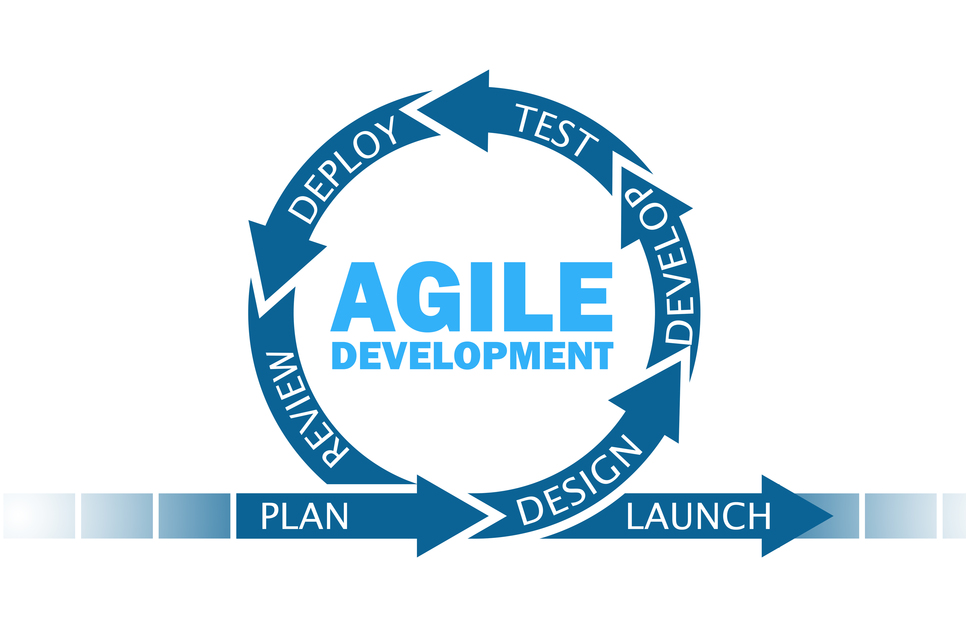
\includegraphics[width=0.7\linewidth]{immagini/agile}
			\caption{Metologia Agile - Fonte: \url{https://www.cleart.com/what-is-agile-software-development.html}}
			\label{fig:agile}
		\end{figure}
		
	Il punto di partenza di ogni ciclo è il risultato raggiunto con il precedente e il feedback
	ricevuto tramite la presentazione della soluzione raggiunta fin’ora agli stakeholder.
	
	La duranta dello stage è stata di 8 settimane quindi ho pianificato 4 sprint della durata di due settimane:
	\begin{enumerate}
		\item studio delle tecnologie, degli strumenti di sviluppo e del sotware gestionale esistente;
		\item progettazione, codifica e testing del modulo Banche;
		\item progettazione, codifica e testing del modulo Fatture Attive;
		\item progettazione, codifica e testing del modulo Fatture Passive.
	\end{enumerate}
			

\section{Tecnologie adottate}

	\subsection{Django}
		Per creare il back-end delle applicazioni rivolte ai clienti, il dipartimento utilizza Django,
		un framework di alto livello gratuito e open source scritto in Python, che incoraggia lo
		sviluppo veloce e pulito di applicazioni web.
	

\section{Progettazione}
	L’architettura del prodotto si suddivide in due macro componenti:
	\begin{itemize}
		\item \textbf{Client}: rappresenta l’applicativo desktop attraverso cui gli utenti interagis-
		cono con il front-end dell’applicazione. Il progetto si focalizza sullo sviluppo
		di questa componente.
		\item \textbf{Server}: rappresenta il sistema remoto che si occupa di calcolare e rispondere
		alle richieste del Client, viene implementato tramite il back-end. Lo sviluppo
		di questa componente non è pertinente al progetto ed è assegnata ad altri
		dipendenti dell’azienda.
	\end{itemize}

	Il Client interagirà con il Server tramite delle API messe pubblicate, che sono
	conformi ai principi REST.
	
	Tecnologie adottate
	
	Strumenti

\section{Realizzazione}

\section{Verifica e Validazione}
	\subsection{Metriche}
	
	\subsection{Risultati}

\section{Risultato}
	\subsection{Modifiche Migliorative}
